% !TeX root = ./../memoria.tex
% Chapter Template

\chapter{Ensayos y resultados} % Main chapter title

\label{Capitulo4}

En este capítulo se detallan las pruebas que fueron realizadas sobre los distintos módulos de hardware y software que componen al robot así como los resultados de las pruebas de campo que se llevaron a cabo.

\section{Pruebas unitarias en el robot}
que le siguieron
En esta sección se describen las pruebas funcionales ejecutadas sobre cada uno de los módulos que componen el robot de manera aislada. Esto permitió encontrar problemas puntuales y reducir las fuentes de error para las pruebas de integración que le siguieron.

\subsection{Validación de conexión bidireccional Roomba-microcontrolador}

Descripción del setup del microcontrolador usando 2 conexiones UART simultáneas.

Envío de comandos de: conexión, desconexión.

\begin{figure}[ht]
    \centering
    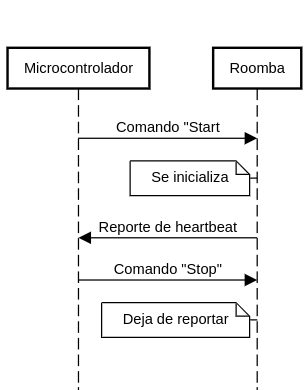
\includegraphics[scale=0.6]{./Figures/comm_test2.png}
    \caption{Diagrama de secuencias ejecutadas durante el test de comunicación entre el microcontrolador y el Roomba.}
    \label{fig:secMicroRoomba}
\end{figure}

\subsection{Validación de conexión bidireccional microcontrolador-ROS}

Descripción de la conexión con ROS usando un mensaje de ``ping'' con una doble confirmación. En el diagrama de la figura \ref{fig:secMicroROS} se muestra la secuencia de acciones llevadas a cabo para la prueba.

\begin{figure}[ht]
    \centering
    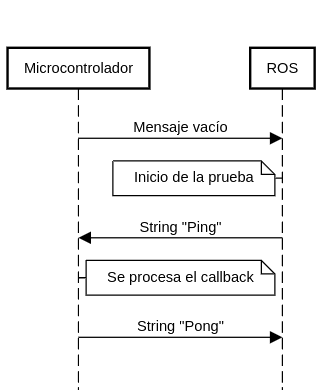
\includegraphics[scale=0.6]{./Figures/comm_test1.png}
    \caption{Diagrama de secuencias ejecutadas durante el test entre el microcontrolador y una PC con ROS.}
    \label{fig:secMicroROS}
\end{figure}

\subsection{Validación de frenado de emergencia}

El Roomba funciona de una manera tal que si recibe un comando de velocidad, este se aplica al robot por tiempo indefinido. Con el fin de prevenir riesgos, se implementó en el controlador un sistema de frenado de emergencia que responde a los siguientes pasos:

\begin{itemize}
    \item Se activa en cuanto se recibe un comando de velocidad distinto de cero.
    \item Se activa una tarea periódica, ejecutada cada 500 ms en donde se comprueba la existencia de al menos un mensaje nuevo en el tópico /cmd\_vel.
    \item En caso que no haya ningún mensaje, la tarea envía la orden de detener el robot.
\end{itemize}

\subsection{Validación de desplazamiento efectivo del robot}

El Roomba implementa su propio sistema de control interno para llevar sus ruedas hasta el \textit{set point} requerido por los comandos de velocidad. En vista de que esta funcionalidad resulta crítica para el sistema, se desarrolló un caso de prueba especial para velocidades tanto positivas como negativas que se describe a continuación:

\begin{itemize}
    \item mediante un script de Python conectado a ROS se envió un comando que establece la velocidad de ambas ruedas a 0,1 m/s por una duración de 10 s es decir, el equivalente a un desplazamiento lineal de 1 m.
    \item mediante una cinta métrica se compararon los valores esperados con el desplazamiento lineal real.
\end{itemize}

Un análisis cualitativo de los resultados expuestos en la tabla \ref{tab:desplazamientoRobot} evidencia que el sistema de control de velocidades interno del Roomba asume que la masa del robot es constante y no toma en cuenta el peso del hardware agregado. Como consecuencia los comandos para mover el robot muestran un porcentaje de error importante.

\begin{table}[!htbp]
    \centering
    \caption[Desplazamiento robot]{Resultados de validación de desplazamiento efectivo del robot}
    \begin{tabular}{lccc}
        \toprule
        \textbf{Movimiento} & \textbf{Desplazamiento} & \textbf{Desplazamiento} & \textbf{Error}    \\
                            & \textbf{esperado}       & \textbf{obtenido}       & \textbf{obtenido} \\
        \midrule
        Lineal positivo 1 m & 1,0 m                   & 0,98 m                  & 2 \%              \\
        Lineal negativo 1 m & -1,0 m                  & -0,96 m                 & 4 \%              \\
        \bottomrule
        \hline
    \end{tabular}
    \label{tab:desplazamientoRobot}
\end{table}

Como medida paliativa se decidió no utilizar el robot en modo reversa para las tareas de mapeo de manera a reducir el error acumulativo.

\subsection{Validación de lectura de encoders}

Dado que es posible obtener las lecturas crudas de los encoders del robot, se realizó la comprobación siguiente de manera similar a la prueba anterior:

\begin{itemize}
    \item mediante un script de Python conectado a ROS se envió un comando de velocidad que establece la velocidad de ambas ruedas a 0.1 m/s por una duración de 10 s es decir, el equivalente a un desplazamiento de 1 m.
    \item mediante los encoders se obtuvo la cantidad de \textit{ticks} o cuentas ocurridas durante dicho periodo.
    \item se calculó el desplazamiento estimado mediante la siguiente fórmula obtenida a partir del documento de especificaciones del fabricante \citep{PAPER:5}:
          \begin{equation}
              Disancia = nTicks / 4498,9125
          \end{equation}

\end{itemize}

Los resultados expuestos en la tabla \ref{tab:lecturaEncoders} muestran ciertas similitudes con los resultados de la prueba anterior en el sentido que el robot reporta un movimiento más ``corto'' que el que le fue comandado. Dado que el número de \textit{ticks} de la rueda izquierda es mayor que el de la derecha, es correcto asumir que el robot describió un movimiento curvilíneo con radio de giro hacia la derecha, lo que pudo comprobarse por el autor al observar la posición del robot al final de la prueba.

\begin{table}[!htbp]
    \centering
    \caption[Lectura de encoders]{Resultados de validación de lectura de encoders}
    \begin{tabular}{lcccccc}
        \toprule
        \multirow{2}{*}{\textbf{Movimiento}} & \multicolumn{2}{l}{\textbf{Ticks esperados}} & \multicolumn{2}{l}{\textbf{Ticks obtenidos}} & \multicolumn{2}{l}{\textbf{Error obtenido}}                                                 \\
                                             & \textbf{Izq.}                                & \textbf{Der.}                                & \textbf{Izq.}                               & \textbf{Der.} & \textbf{Izq.} & \textbf{Der.} \\
        \midrule
        Lineal positivo 1 m                  & 2250                                         & 2250                                         & 2201                                        & 2137          & 2,22 \%       & 5,28 \%       \\
        Lineal negativo 1 m                  & 2250                                         & 2250                                         & 2194                                        & 2103          & 2,55 \%       & 6,99 \%       \\
        \bottomrule
        \hline
    \end{tabular}
    \label{tab:lecturaEncoders}
\end{table}

\subsection{Validación de lecturas crudas de la IMU}

Esta prueba consistió en graficar las lecturas de las seis variables registradas por el sensor durante una secuencia de tres movimientos a la que fue sometido.

Para esta prueba se partió de un estado inicial con la IMU quieta, con el plano definido por sus ejes $(X,Y)$ en posición normal al vector de aceleración de la gravedad (que apunta al centro de la Tierra). Para todas las pruebas se utilizó la convención ``North-East-Down'' \protect\footnotemark que el sensor adopta por defecto.

\footnotetext{Coordenadas locales del plano tangente NED: \url{https://en.wikipedia.org/wiki/Local\_tangent\_plane\_coordinates}}

Basado en las lecturas del acelerómetro de la figura \ref{fig:aceleracionLineal} se describen las observaciones realizadas:

\begin{itemize}
    \item en la primera columna se observa el vector de aceleración de la gravedad de aproximadamente 9,8 $m/s^2$ apuntando en la dirección negativa del eje $Z$.
    \item en la segunda columna se observa el mismo vector de aceleración, esta vez trasladado en dirección del eje $X$ negativo.
    \item finalemente en la tercera columna se observa al vector transladado en dirección al eje $Y$ negativo.
\end{itemize}


\begin{figure}[ht]
    \centering
    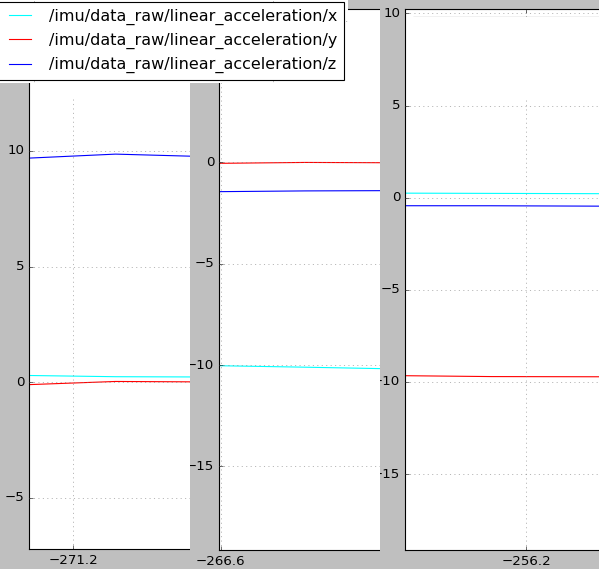
\includegraphics[scale=0.4]{./Figures/linear_acceleration.png}
    \caption{Gráfico de aceleraciones lineales sobre cada uno de los ejes registrados durante las tres posiciones de prueba.}
    \label{fig:aceleracionLineal}
\end{figure}


Para las gráficas del giroscopio se procedió con la misma metodología utilizada para el acelerómetro. La diferencia en estas pruebas radica en que los valores medidos por el giroscopio son instantáneos, ya que corresponden a velocidades angulares alrededor de los ejes durante los movimientos efectuados, y desaparecen al dejar de mover la IMU. Por este motivo se presentan seis gráficas que fueron distribuidas en las figuras \ref{fig:velocidadAngular1} y \ref{fig:velocidadAngular2} de izquierda a derecha, donde se muestran los valores adoptados por los tres ejes del giroscopio durante los movimientos descriptos a continuación:

\begin{enumerate}
    \item giro alrededor del eje $Y$ en sentido antihorario.
    \item giro alrededor del eje $Y$ en sentido horario.
    \item giro alrededor del eje $X$ en sentido antihorario.
    \item giro alrededor del eje $X$ en sentido horario.
    \item giro alrededor del eje $Z$ en sentido antihorario.
    \item giro alrededor del eje $Z$ en sentido horario.
\end{enumerate}

\begin{figure}[ht]
    \centering
    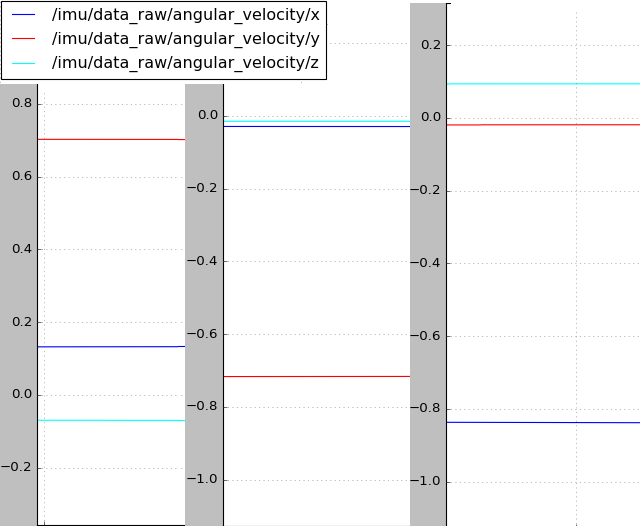
\includegraphics[scale=0.42]{./Figures/angular_velocity_1.png}
    \caption{Gráfico de velocidades angulares durante los movimientos 1, 2 y 3.}
    \label{fig:velocidadAngular1}
\end{figure}

\begin{figure}[ht]
    \centering
    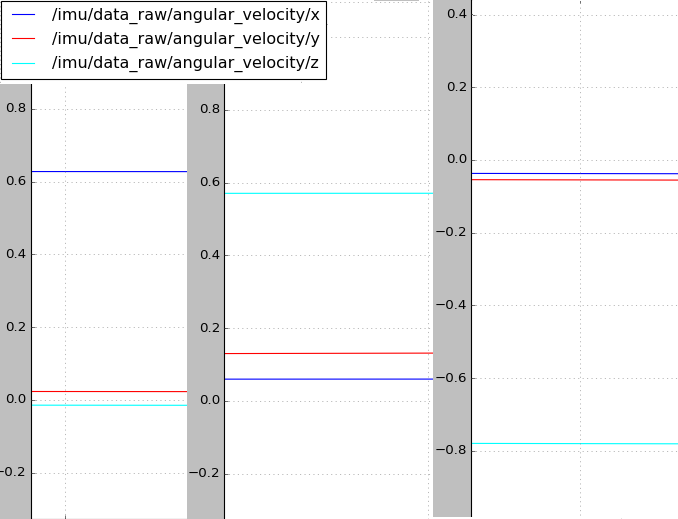
\includegraphics[scale=0.42]{./Figures/angular_velocity_2.png}
    \caption{Gráfico de velocidades angulares durante los movimientos 4, 5 y 6.}
    \label{fig:velocidadAngular2}
\end{figure}


\section{Pruebas unitarias en la PC}

En esta sección se describen las pruebas realizadas sobre los resultados arrojados por los componentes de software ejecutados en la PC. Estos se utilizan para procesar los datos crudos arrojados por los sensores y generar información en un formato aprovechable por ROS.

\subsection{Validación de cálculo de odometría con encoders}

Esta prueba tuvo como objetivo validar el correcto funcionamiento del programa lubo\_odom\_node, que consume las lecturas de encoders y realiza con estas una estimación de la posición y orientación del robot en un plano $(X,Y)$.

Para la validación de esta característica, la prueba se realizó siguiendo los siguientes pasos:
\begin{enumerate}
    \item se marcó la pose inicial del robot en el suelo.
    \item se comandaó el robot con un \textit{joystick} a una velocidad aproximada de 0,1 $m/s$.
    \item se movió el robot aproximadamente 1 $m$ hacia adelante.
    \item se hizo girar el robot aproximadamente 90 grados.
    \item se movió nuevamente el robot aproximadamente 1 $m$ hacia adelante.
    \item se midió la distancia lineal entre el punto de inicio y el punto final del robot.
    \item se obtuvieron las componentes en $X$ e $Y$ del vector de distancia trazado en el punto anterior.
    \item se comparararon estas medidas con los valores arrojados por la odometría, y con esto se calculó el error. Esta información se expone en la tabla \ref{tab:odometriaEncoders}.
\end{enumerate}

\begin{table}[!htbp]
    \centering
    \caption[Odometria de encoders]{Resultados de validación de odometría de encoders}
    \begin{tabular}{lccc}
        \toprule
        \textbf{Variable}  & \textbf{Medición esperada} & \textbf{Medición reportada} & \textbf{Error obtenido} \\
        \midrule
        Posición en $X$    & 1 m                        & 1,04 m                      & 4 \%                    \\
        Posición en $Y$    & 1 m                        & 0,8 m                       & 20 \%                   \\
        Orientación en $Z$ & -0,785 rad                 & -0,729 rad                  & 7,73 \%                 \\
        \bottomrule
        \hline
    \end{tabular}
    \label{tab:odometriaEncoders}
\end{table}

% \subsection{Validación de estimador de pose con filtro Madwick para IMU}

% El IMU MPU6050 no ofrece medición de campo magnético, por este motivo la información que provee resulta limitada e insuficiente para estimar la orientación absoluta del dispositivo.
% Existen varias soluciones diferentes distintas para esta problemática pero para este trabajo se eligió utilizar un estimador de pose, es decir, un filtro especial que toma la información en bruto de acelerómetro y giroscopio y a su salida provee además de los valores filtrados de sus entradas, una estimación de la orientación del sensor.

% Descripción de los resultados arrojados por la IMU MPU6050 en bruto. Gráfico de rqt\_plot
% Resultados arrojados por las mismas mediciones, esta vez con el filtro activado.

\subsection{Validación de estimador de odometría con encoders + IMU}

Gracias a la aplicación de un Filtro de Kalman Extendido por parte del paquete robot\_localization, fue posible combinar la información provista por el cálculo de odometría de encoders junto con el estimador de pose de la IMU.

Este procedimiento consistió en comparar los resultados obtenidos con la prueba de odometría de encoders pura del punto anterior y la estimación de odometria resultante de combinar este valor con la pose de la IMU. El procedimiento ejecutado fue el mismo que se utilizó en el punto anterior y los resultados se exponen en la tabla \ref{tab:odometriaFusion}.

\begin{table}[!htbp]
    \centering
    \caption[Fusión de odometría con IMU]{Resultados de validación del estimador de odometría mediante la fusión de datos de encoders e IMU.}
    \begin{tabular}{lccc}
        \toprule
        \textbf{Variable}  & \textbf{Medición esperada} & \textbf{Medición reportada} & \textbf{Error obtenido} \\
        \midrule
        Posición en $X$    & 1 m                        & 1,01 m                      & 1 \%                    \\
        Posición en $Y$    & 1 m                        & 0,98 m                      & 2 \%                    \\
        Orientación en $Z$ & -0,785 rad                 & -0,786 rad                  & 0,13 \%                 \\
        \bottomrule
        \hline
    \end{tabular}
    \label{tab:odometriaFusion}
\end{table}

\newpage

Gracias a que ambos tests se encargan de reproducir el mismo escenario fue posible comparar ambos resultados y obtener el porcentaje de mejora ofrecido por la fusión de datos sobre el error absoluto. Los resultados de esta comparación se pueden apreciar en la tabla \ref{tab:comparacionOdom}.

\begin{table}[!htbp]
    \centering
    \centering
    \caption[Comparacion de calculos de odometría]{Resultados obtenidos al comparar las lecturas arrojadas por la odometría de encoders ``pura'' y la odometría resultante de la fusión de encoders e IMU.}
    \begin{tabular}{lccc}
        \toprule
        \textbf{Variable}  & \textbf{Técnica 1} & \textbf{Técnica 2} & \textbf{Porcentaje de mejora} \\
        \midrule
        Posición en $X$    & 1,04 m             & 1,01 m             & \textasciitilde300 \%         \\
        Posición en $Y$    & 0,8 m              & 0,98 m             & \textasciitilde1000 \%        \\
        Orientación en $Z$ & -0,729 rad         & -0,786 rad         & \textasciitilde6000 \%        \\
        \bottomrule
    \end{tabular}
    \label{tab:comparacionOdom}
\end{table}


\section{Pruebas de integración en campo}

En esta sección se describen las pruebas funcionales ejecutadas sobre cada uno de los módulos que componen el robot de manera aislada. Esto permitió encontrar problemas puntuales y reducir las fuentes de error para las pruebas de integración.

\subsection{Generación de mapa con gmapping}

Esta prueba consistió en la generación de un mapa del tipo \textit{occupancy grid} o mapa de ocupación. Este mapa consiste en una representación similar a la de un plano en dos dimensiones como los utilizados en arquitectura. Los puntos en negro representan una sección ``ocupada'' mientras que los píxeles blancos representan un área libre.


Para que el resultado obtenido a partir de este procedimiento fuera lo suficientemente preciso como para utilizarse en la tarea de localizar al robot fue necesario que la fuente de odometría fuera muy precisa, motivo por el que resultó indispensable el uso de la fuente de odometría filtrada con información de la IMU.

En las figuras \ref{fig:mapaFeo} se puede apreciar el mapa obtenido a partir de la odometría de encoders ``pura''. Este primer mapa resulta totalmente inutilizable para tareas de navegación puesto que no refleja la morfología real del recinto. Por el contrario, el mapa de la figura \ref{fig:mapaLindo} se generó utilizando la fuente de odometría filtrada con IMU. A pesar de sus restricciones, este último mapa resultó suficiente para las tareas de localización y navegación del robot.


\begin{figure}[ht]
    \centering
    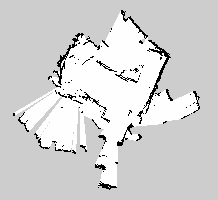
\includegraphics[scale=1.0]{./Figures/mapa_feo.png}
    \caption{Mapa obtenido utilizando odometría de encoders ``pura''.}
    \label{fig:mapaFeo}
\end{figure}

\begin{figure}[ht]
    \centering
    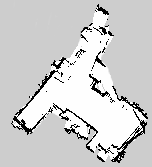
\includegraphics[scale=1.2]{./Figures/mapa_lindo.png}
    \caption{Mapa obtenido utilizando odometría filtrada.}
    \label{fig:mapaLindo}
\end{figure}


%TODO: agregar imagenes de 1) Mapa horrible sin ekf 2) mapita decente con ekf.

\subsection{Localización en mapa con amcl}

% Tal como se describió en la sección \ref{sec:amcl}, amcl es un paquete para ROS que provee al robot la capacidad de encontrar su posición y orientación de un mapa previamente provisto. Esta prueba consistió en la utilización del mapa generado de la sala de estar del departamento del autor. Este fue provisto a la herramienta amcl mediante el servidor de parámetros de ROS y luego se procedió a teleoperar el robot mediante un \textit{joystick} inalámbrico. El procedimiento utilizado fue el siguiente:
Amcl es un paquete para ROS que provee al robot la capacidad de encontrar su posición y orientación de un mapa previamente provisto. Esta prueba consistió en la utilización del mapa generado de la sala de estar del departamento del autor. Este fue provisto a la herramienta amcl mediante el servidor de parámetros de ROS y luego se procedió a teleoperar el robot mediante un \textit{joystick} inalámbrico. El procedimiento utilizado fue el siguiente:

\begin{enumerate}
    \item se colocó el robot en una pose aleatoria en el mapa como se muestra en la figura \ref{fig:sinLocalizar}.
    \item por medio del \textit{joystick} se hizo girar al robot en círculos en sentido horario hasta completar dos vueltas completas de 360 grados a una velocidad angular aproximada de 0,5 rad/s.
    \item se aplicó el mismo procedimiento para un giro en sentido anti-horario.
\end{enumerate}


\begin{figure}[ht]
    \centering
    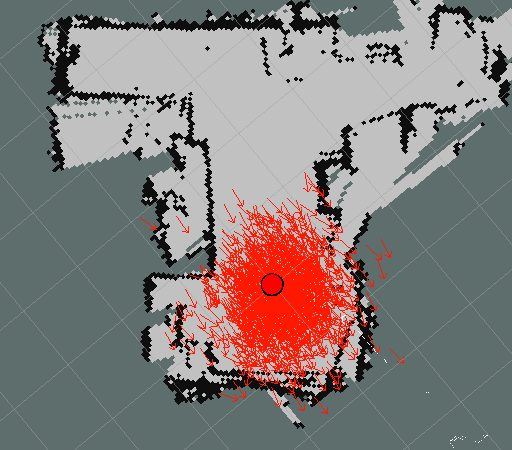
\includegraphics[scale=0.4]{./Figures/sin_localizar.png}
    \caption{Captura de pantalla de RViz con el robot aún sin localizarse. Las flechas rojas muestran las posibles poses del robot en el mapa.}
    \label{fig:sinLocalizar}
\end{figure}

El resultado final se puede apreciar en la figura \ref{fig:robotLocalizado}. En esta imagen, tanto la posición en $X$ e $Y$ del robot con respecto al mapa han sido estimadas y así también su orientación respecto al eje $Z$.

\begin{figure}[ht]
    \centering
    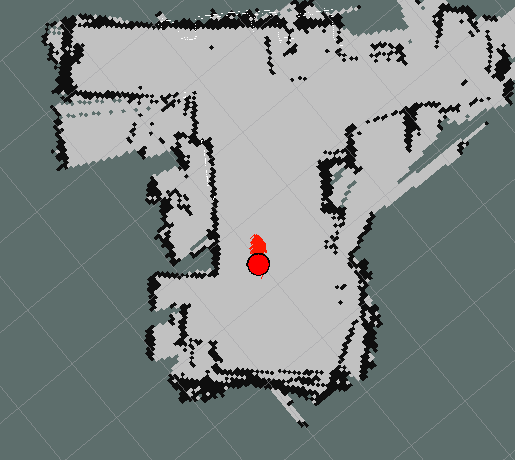
\includegraphics[scale=0.4]{./Figures/robot_localizado.png}
    \caption{Captura de pantalla de RViz con el robot localizado. En este momento las flechas rojas han convergido hacia una misma región donde se estima que se encuentra el robot.}
    \label{fig:robotLocalizado}
\end{figure}

\subsection{Navegación en mapa con move\_base}

% Así como se describe en la sección \ref{sec:move_base}, move\_base provee la funcionalidad necesaria para mover al robot dentro del mapa provisto, para lo cual la herramienta se encarga de calcular una ruta de navegación desde el punto en que el robot se encuentra al momento de enviarse la orden y otro punto cualquiera del mapa.
El paquete move\_base provee la funcionalidad necesaria para mover al robot dentro del mapa provisto, para lo cual la herramienta se encarga de calcular una ruta de navegación desde el punto en que el robot se encuentra al momento de enviarse la orden y otro punto cualquiera del mapa.

Esta prueba consistió en indicar a la herramienta que deseábamos mover el robot de un punto a otro en el mapa. Para esto fue necesario cumplir con ciertos requisitos previos:

\begin{enumerate}
    \item un mapa estático debió ser provisto al servidor de mapas de ROS.
    \item el robot debió encontrarse previamente localizado en el mapa.
\end{enumerate}

El envío de consigna se realiza mediante la herramienta RViz, que se representa mediante un vector de color verde en el mapa. Su punto de origen representa la posición deseada mientras que su dirección representa la orientación final del robot. En las figuras \ref{fig:comandoNavegación} y \ref{fig:robotEnSetpoint} se puede apreciar al robot en su punto de inicio al momento de recibir la orden de navegación y al robot ya en su punto de destino, respectivamente.


\begin{figure}[ht]
    \centering
    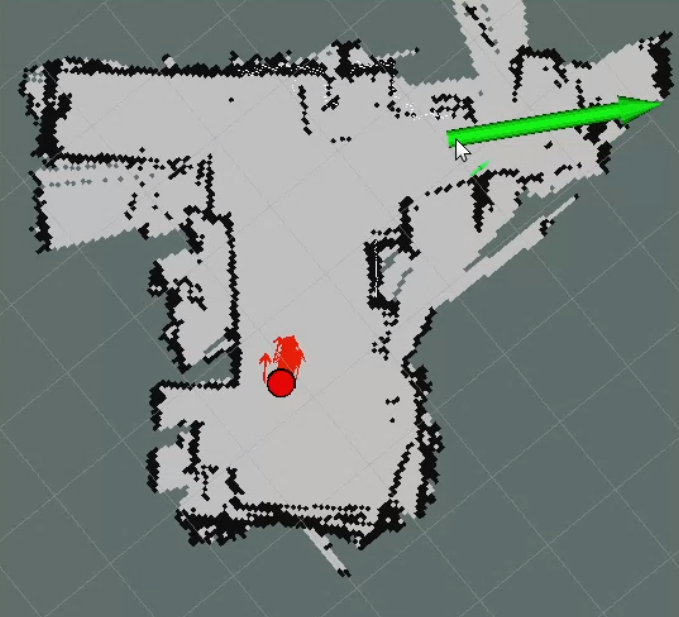
\includegraphics[scale=0.35]{./Figures/comando_navegacion.png}
    \caption{Captura de pantalla de RViz con el robot localizado al momento de recibir una orden de navegación.}
    \label{fig:comandoNavegación}
\end{figure}


\begin{figure}[ht]
    \centering
    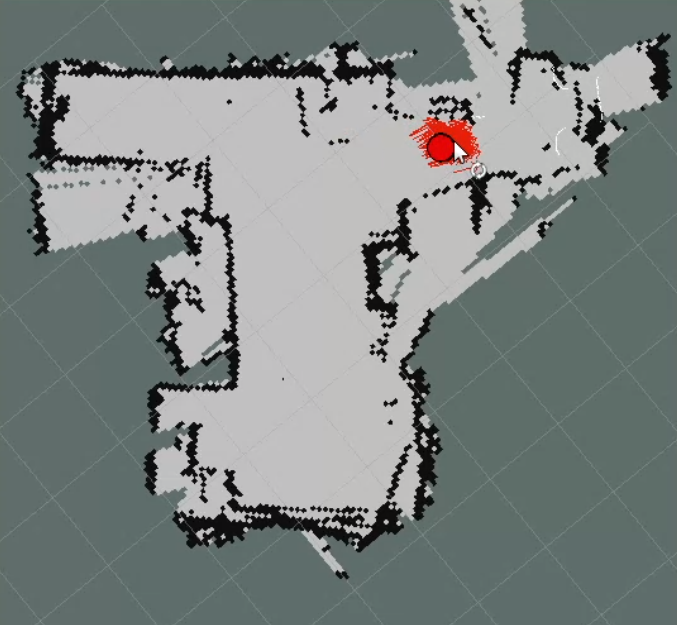
\includegraphics[scale=0.35]{./Figures/robot_en_setpoint.png}
    \caption{Captura de pantalla de RViz con el robot en su punto de consigna.}
    \label{fig:robotEnSetpoint}
\end{figure}